% ========================================
%	Header einbinden
% ========================================

\documentclass[bibtotoc,titlepage]{scrartcl}

% Deutsche Spracheinstellungen
\usepackage[ngerman,german]{babel, varioref}
\usepackage[T1]{fontenc}
\usepackage[utf8]{inputenc}

%\usepackage{marvosym}

\usepackage{amsfonts}
\usepackage{amssymb}
\usepackage{amsmath}
\usepackage{amscd}
\usepackage{amstext}
\usepackage{float}
\usepackage{caption}
\usepackage{wrapfig}
\usepackage{setspace}
\usepackage{threeparttable}
\usepackage{footnote}

\newfloat{formel}{htbp}{for}
\floatname{formel}{Formel}


\usepackage{longtable}

%\usepackage{bibgerm}

\usepackage{footnpag}

\usepackage{ifthen}                 %%% package for conditionals in TeX
\usepackage[amssymb]{SIunits}
%Fr textumflossene Bilder und Tablellen
%\usepackage{floatflt} - veraltet

%Fr Testzwecke aktivieren, zeigt labels und refs im Text an.
%\usepackage{showkeys}

% Abstand zwischen zwei Abs�zen nach DIN (1,5 Zeilen)
% \setlength{\parskip}{1.5ex plus0.5ex minus0.5ex}

% Einrckung am Anfang eines neuen Absatzes nach DIN (keine)
%\setlength{\parindent}{0pt}

% R�der definieren
% \setlength{\oddsidemargin}{0.3cm}
% \setlength{\textwidth}{15.6cm}

% bessere Bildunterschriften
%\usepackage[center]{caption2}


% Probleml�ungen beim Umgang mit Gleitumgebungen
\usepackage{float}

% Nummeriert bis zur Strukturstufe 3 (also <section>, <subsection> und <subsubsection>)
%\setcounter{secnumdepth}{3}

% Fhrt das Inhaltsverzeichnis bis zur Strukturstufe 3
%\setcounter{tocdepth}{3}

\usepackage{exscale}

\newenvironment{dsm} {\begin{displaymath}} {\end{displaymath}}
\newenvironment{vars} {\begin{center}\scriptsize} {\normalsize \end{center}}


\newcommand {\en} {\varepsilon_0}               % Epsilon-Null aus der Elektrodynamik
\newcommand {\lap} {\; \mathbf{\Delta}}         % Laplace-Operator
\newcommand {\R} { \mathbb{R} }                 % Menge der reellen Zahlen
\newcommand {\e} { \ \mathbf{e} }               % Eulersche Zahl
\renewcommand {\i} { \mathbf{i} }               % komplexe Zahl i
\newcommand {\N} { \mathbb{N} }                 % Menge der nat. Zahlen
\newcommand {\C} { \mathbb{C} }                 % Menge der kompl. Zahlen
\newcommand {\Z} { \mathbb{Z} }                 % Menge der kompl. Zahlen
\newcommand {\limi}[1]{\lim_{#1 \rightarrow \infty}} % Limes unendlich
\newcommand {\sumi}[1]{\sum_{#1=0}^\infty}
\newcommand {\rot} {\; \mathrm{rot} \,}         % Rotation
\newcommand {\grad} {\; \mathrm{grad} \,}       % Gradient
\newcommand {\dive} {\; \mathrm{div} \,}        % Divergenz
\newcommand {\dx} {\; \mathrm{d} }              % Differential d
\newcommand {\cotanh} {\; \mathrm{cotanh} \,}   %Cotangenshyperbolicus
\newcommand {\asinh} {\; \mathrm{areasinh} \,}  %Area-Sinus-Hyp.
\newcommand {\acosh} {\; \mathrm{areacosh} \,}  %Area-Cosinus-H.
\newcommand {\atanh} {\; \mathrm{areatanh} \,}  %Area Tangens-H.
\newcommand {\acoth} {\; \mathrm{areacoth} \,}  % Area-cotangens
\newcommand {\Sp} {\; \mathrm{Sp} \,}
\newcommand {\mbe} {\stackrel{\text{!}}{=}}     %Must Be Equal
\newcommand{\qed} { \hfill $\square$\\}
\renewcommand{\i} {\imath}
\def\captionsngerman{\def\figurename{\textbf{Abb.}}}

%%%%%%%%%%%%%%%%%%%%%%%%%%%%%%%%%%%%%%%%%%%%%%%%%%%%%%%%%%%%%%%%%%%%%%%%%%%%
% SWITCH FOR PDFLATEX or LATEX
%%%%%%%%%%%%%%%%%%%%%%%%%%%%%%%%%%%%%%%%%%%%%%%%%%%%%%%%%%%%%%%%%%%%%%%%%%%%
%%%
\ifx\pdfoutput\undefined %%%%%%%%%%%%%%%%%%%%%%%%%%%%%%%%%%%%%%%%% LATEX %%%
%%%
\usepackage[dvips]{graphicx}       %%% graphics for dvips
\DeclareGraphicsExtensions{.eps,.ps}   %%% standard extension for included graphics
\usepackage[ps2pdf]{thumbpdf}      %%% thumbnails for ps2pdf
\usepackage[ps2pdf,                %%% hyper-references for ps2pdf
bookmarks=true,%                   %%% generate bookmarks ...
bookmarksnumbered=true,%           %%% ... with numbers
hypertexnames=false,%              %%% needed for correct links to figures !!!
breaklinks=true,%                  %%% breaks lines, but links are very small
linkbordercolor={0 0 1},%          %%% blue frames around links
pdfborder={0 0 112.0}]{hyperref}%  %%% border-width of frames
%                                      will be multiplied with 0.009 by ps2pdf
%
\hypersetup{ pdfauthor   = {Hannes Franke; Julius Tilly},
pdftitle    = {V301 Innenwiderstand und Leistungsanpassung}, pdfsubject  = {Protokoll FP}, pdfkeywords = {V301, Innenwiderstand, Leistungsanpassung},
pdfcreator  = {LaTeX with hyperref package}, pdfproducer = {dvips
+ ps2pdf} }
%%%
\else %%%%%%%%%%%%%%%%%%%%%%%%%%%%%%%%%%%%%%%%%%%%%%%%%%%%%%%%%% PDFLATEX %%%
%%%
\usepackage[pdftex]{graphicx}      %%% graphics for pdfLaTeX
\DeclareGraphicsExtensions{.pdf}   %%% standard extension for included graphics
\usepackage[pdftex]{thumbpdf}      %%% thumbnails for pdflatex
\usepackage[pdftex,                %%% hyper-references for pdflatex
bookmarks=true,%                   %%% generate bookmarks ...
bookmarksnumbered=true,%           %%% ... with numbers
hypertexnames=false,%              %%% needed for correct links to figures !!!
breaklinks=true,%                  %%% break links if exceeding a single line
linkbordercolor={0 0 1},
linktocpage]{hyperref} %%% blue frames around links
%                                  %%% pdfborder={0 0 1} is the default
\hypersetup{
pdftitle    = {V301 Innenwiderstand und Leistungsanpassung}, 
pdfsubject  = {Protokoll AP}, 
pdfkeywords = {V301, Innenwiderstand, Leistungsanpassung},
pdfsubject  = {Protokoll AP},
pdfkeywords = {V301, Innenwiderstand, Leistungsanpassung}}
%                                  %%% pdfcreator, pdfproducer,
%                                      and CreationDate are automatically set
%                                      by pdflatex !!!
\pdfadjustspacing=1                %%% force LaTeX-like character spacing
\usepackage{epstopdf}
%
\fi %%%%%%%%%%%%%%%%%%%%%%%%%%%%%%%%%%%%%%%%%%%%%%%%%%% END OF CONDITION %%%
%%%%%%%%%%%%%%%%%%%%%%%%%%%%%%%%%%%%%%%%%%%%%%%%%%%%%%%%%%%%%%%%%%%%%%%%%%%%
% seitliche Tabellen und Abbildungen
%\usepackage{rotating}
\usepackage{ae}
\usepackage{
  array,
  booktabs,
  dcolumn
}
\makeatletter 
  \renewenvironment{figure}[1][] {% 
    \ifthenelse{\equal{#1}{}}{% 
      \@float{figure} 
    }{% 
      \@float{figure}[#1]% 
    }% 
    \centering 
  }{% 
    \end@float 
  } 
  \makeatother 


  \makeatletter 
  \renewenvironment{table}[1][] {% 
    \ifthenelse{\equal{#1}{}}{% 
      \@float{table} 
    }{% 
      \@float{table}[#1]% 
    }% 
    \centering 
  }{% 
    \end@float 
  } 
  \makeatother 
%\usepackage{listings}
%\lstloadlanguages{[Visual]Basic}
%\allowdisplaybreaks[1]
%\usepackage{hycap}
%\usepackage{fancyunits}
\usepackage{multirow}
\usepackage{color}

% ========================================
%	Angaben für das Titelblatt
% ========================================

\title{Versuch 28 - Elektronenspinresonanz\\% Titel des Versuchs 
\large TU Dortmund, Fakultät Physik\\ 
\normalsize Fortgeschrittenen-Praktikum}

\author{Jan Adam\\			% Name Praktikumspartner A
{\small \href{jan.adam@tu-dortmund.de}{jan.adam@tu-dortmund.de}}	% Erzeugt interaktiven einen Link
\and						% um einen weiteren Author hinzuzfügen
Dimitrios Skodras\\					% Name Praktikumspartner B
{\small \href{dimitrios.skodras@tu-dortmund.de}{dimitrios.skodras@tu-dortmund.de}}		% Erzeugt interaktiven einen Link
}
\date{30. April 2014}				% Das Datum der Versuchsdurchführung

% ========================================
%	Das Dokument beginnt
% ========================================

\begin{document}

% ========================================
%	Titelblatt erzeugen
% ========================================

\maketitle					% Jetzt wird die Titelseite erzeugt
\thispagestyle{empty} 				% Weder Kopfzeile noch Fußzeile

% ========================================
%	Der Vorspann
% ========================================

%\newpage					% Wenn Verzeichnisse auf einer neuen Seite beginnen sollen
%\pagestyle{empty}				% Weder Kopf- noch Fußzeile für Verzeichnisse

\tableofcontents

%\newpage					% eine neue Seite
%\thispagestyle{empty}				% Weder Kopf- noch Fußzeile für Verzeichnisse
%\listoffigures					% Abbildungsverzeichnis

%\newpage					% eine neue Seite
%\thispagestyle{empty}				% Weder Kopf- noch Fußzeile für Verzeichnisse
%\listoftables					% Tabellenverzeichnis
\newpage					% eine neue Seite


% ========================================
%	Kapitel
% ========================================

%\section{Einleitung}				% Bei Bedarf

\section{Theorie}
\setcounter{page}{1}
Die Hüllenelektronen eines Atoms, die einen Bahndrehimpuls besitzen, erzeugen auch
ein magnetisches Moment. Laut einiger Experimente haben Elektronen jedoch außerdem einen \glqq Eigendrehimpuls\grqq \, genannt \glqq Spin\grqq, der experimentell zu Tage tritt, wenn der Gesamtdrehimpuls der Elektronenhülle verschwindet. Dies ist klassisch nicht zu erklären, da Elektronen punktförmig sind und keine Ausdehnung haben.\\
In diesem Experiment soll nun versucht werden, den Betrag dieses Drehimpulses zu bestimmen.\\

Mit Überlegungen aus der Quantenmechanik lässt sich das gesuchte Bohrsche Magneton herleiten: Die Stromdichte eines Teilchenstroms aus Elektronen ist 
\begin{align}
\vec{S} = \frac{\hbar}{2im_0} (\Psi^* \nabla \Psi - \Psi \nabla \Psi^*)
\end{align}
Mit $\hbar$ dem Planckschen Wirkungsquantum und $m_0$ der Elektronenmasse.\\

Setzt man für $\Psi$ die Kugelförmige Wellenfunktion des Elektrons ein und integriert über die Querschnittsfläche der Elektronenhülle, so erhält man das Bohrsche Magneton $\mu_B$:
\begin{align}
\mu_B := -\frac{1}{2}\frac{e_0}{m_0}\hbar= (9,274015 \pm 0,000003)\cdot10^{-24} \frac{J}{T}
\end{align}
Neben dem Betrag des Drehimpulses ist auch seine Richtung gequantelt. Bezüglicher einer ausgezeichneten Raumachse kann die Komponente $l_z$ nur ganzzahlige Vielfache von $\hbar$ annehmen:
\begin{align}
l_z=m_l\hbar
\end{align}
Mit $m_l = 0, \pm 1, \pm 2,\cdots , \pm l$\\

Wird dieses magnetische Moment in ein äußeres Magnetfeld eingeführt, so erhält es, abhängig von seiner Ausrichtung, potentielle Energie. Seine Grundenergie $E_0$ spaltet in $2l+1$ Unterniveaus auf, der Zeeman-Effekt wird beobachtet.\\

Der Eigenspin der Elektronen kann, wie im Stern-Gerlach-Versuch sichtbar wird, immer nur zwei Werte annehmen: $m_s=\pm \frac{1}{2}$ und damit folgt für die z-Komponente $S_z$:
\begin{align*}
S_z=m_s\hbar=\pm\frac{1}{2}\hbar
\end{align*}

Das Magnetische Moment wird nun zweckmäßigerweise in Einheiten des Bohrschen Magnetons ausgedrückt
\begin{align*}
\mu S_z=-gm_s\mu_B=-g\frac{1}{2}\mu_B
\end{align*}
der dabei auftretende Proportionalitätsfaktor wird \glqq Landé-Faktor\grqq $g$  genannt. Dieser kann $\neq 1$ sein, wodurch ein anderer Zusammenhang als beim Bahndrehimpuls impliziert wird und der genaue Wert soll im Folgenden berechnet werden.
\section{Durchführung und Aufbau}
Zur Bestimmung des g-Faktors wird die Elektronenspin-Resonanz-Methode (ESR) benutzt. Dazu wird eine Substanz mit freien Elektronen in ein homogenes Magnetfeld eingeführt und das Energieniveau $E_0$ mittels Zeeman-Effekt aufgespalten.\\

\begin{figure}[H]
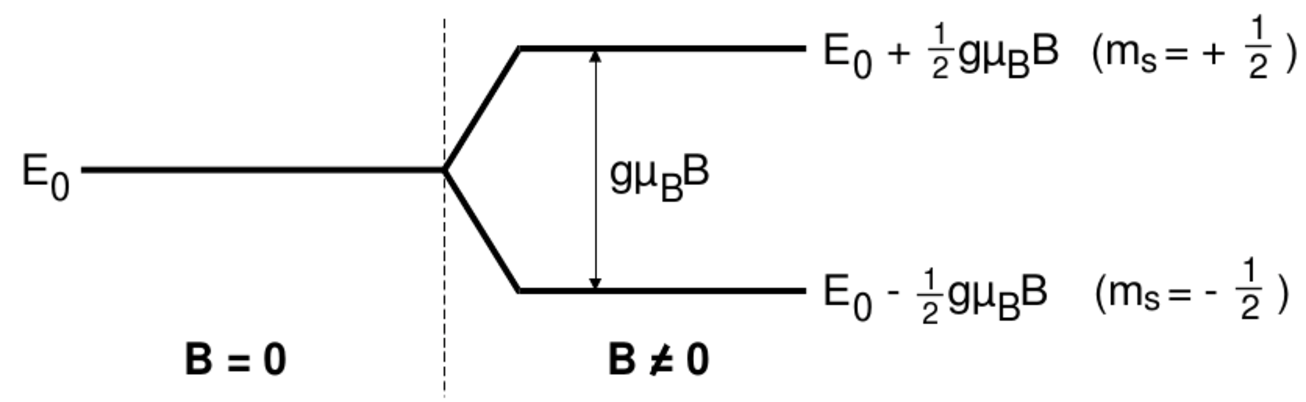
\includegraphics[scale=0.5]{../pics/aufsp.pdf}
\caption{Darstellung der Aufspaltung des Grundniveaus in zwei weitere Niveaus für $B\neq 0$\protect\footnotemark}
\label{pic_aufspaltung}
\end{figure}
\footnotetext{Abbildung aus der Versuchsanleitung entnommen}

Die Energie-Differenz zwischen den beiden Niveaus beträgt dabei
\begin{align}
h\nu = g \mu_B B
\label{eq_energie}
\end{align}

Gemäß der Maxwell-Boltzmann-Verteilung ist der obere Zustand schwächer besetzt als der untere. Durch Einstrahlung von Lichtquanten mit der Differenzenergie von etwa $\hbar\nu \approx 6\cdot10^{-7}eV \Rightarrow \nu \approx 140 \text{MHz}$ bei einem Magnetfeld von $B=10\text{mT}$ kann man die Elektronen in das höhere Niveau anheben, wobei sie ihren Spin umklappen. Dies ist die sog. "Elektronenspin-Resonanz".\\

Das Hochfrequenzfeld wird durch eine kleine Spule induziert. Das homogene Magnetfeld erzeugt eine Helmholtzspule. Wird die Resonanzfrequenz erreicht, so ändert sich die makroskopische Magnetisierung der Probe und damit die Impendanz der HF-Spule. Diese Verstimmung wird an der angeschlossenen Brückenschaltung durch eine Differenz-Spannung sichtbar, die auf einem empfindlichen Messinstrument abgelesen werden kann.

In Abbildung \ref{pic_aufbau} ist der Aufbau der Messapparatur zu erkennen.
\begin{figure}[H]
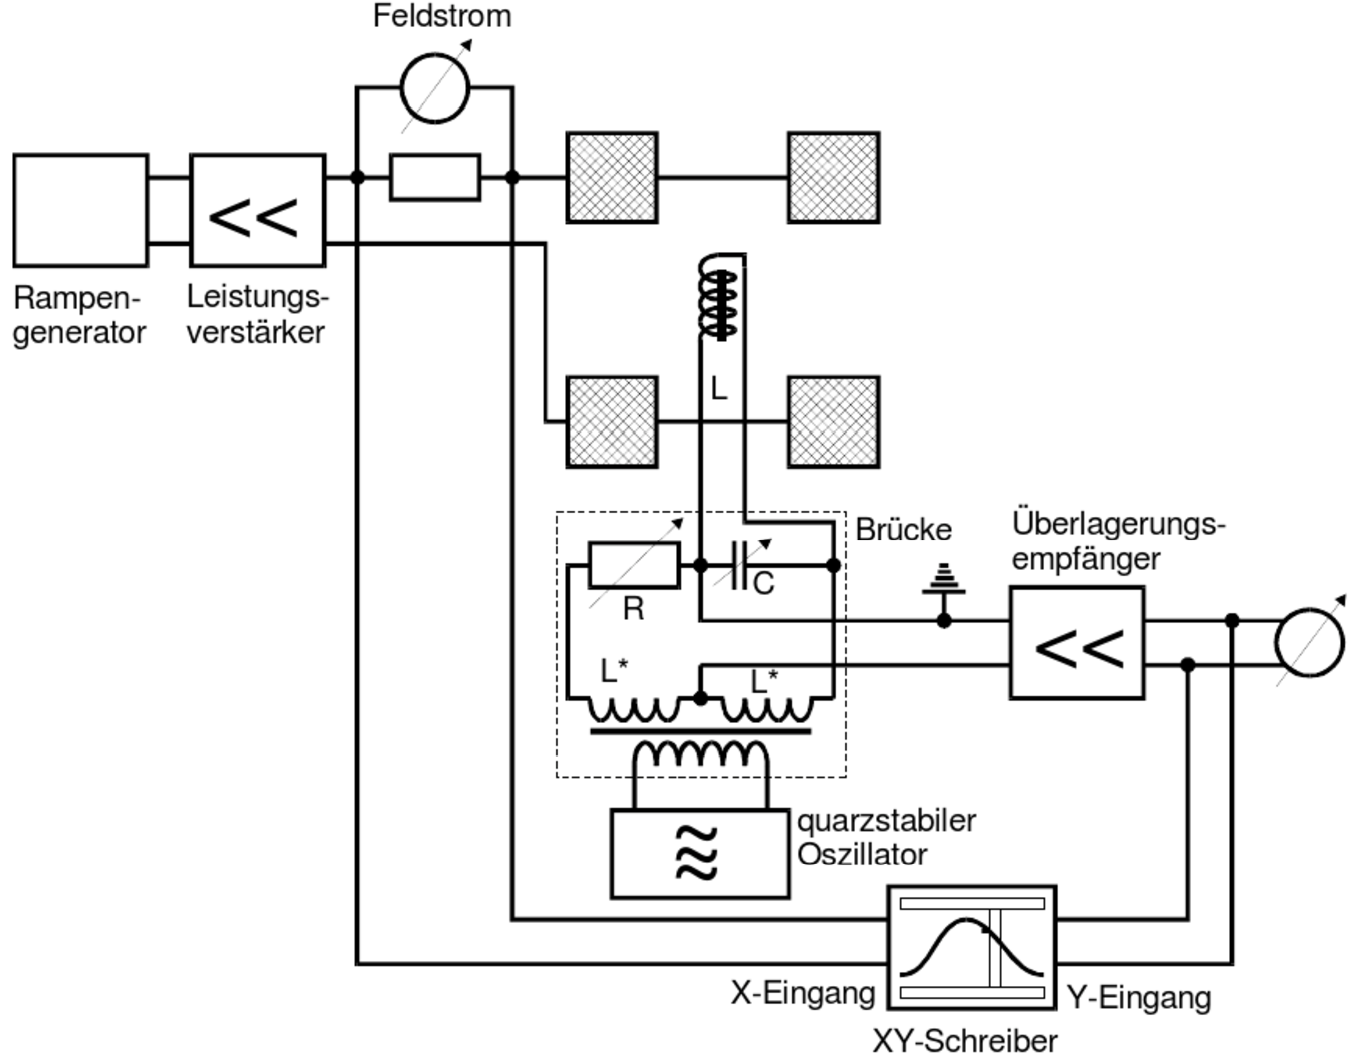
\includegraphics[scale=0.4]{../pics/aufbau.pdf}
\caption{Aufbau der im Versuch verwendeten Messapparatur\protect\footnotemark[2]}
\label{pic_aufbau}
\end{figure}
\footnotetext[2]{Abbildung aus der Versuchsanleitung entnommen}

Die Brückenspannung wird nun verstärkt, gefiltert und zusammen mit dem Output eines Rampengenerators für die Spulenspannung an einen X-Y-Schreiber angeschlossen. Im Idealfall sollte eine Resonanz in Form von Abbildung \ref{pic_resonanz} 
\begin{figure}[H]
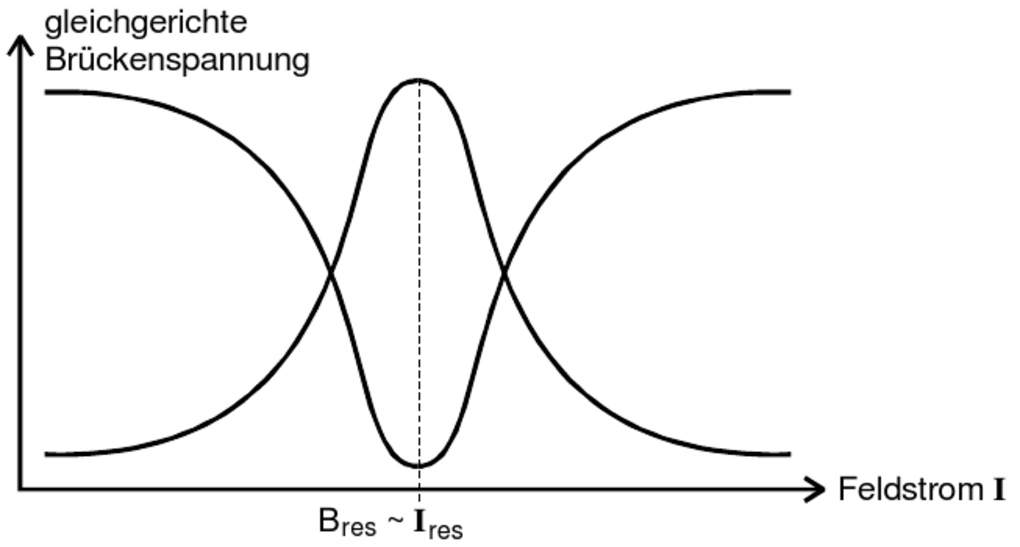
\includegraphics[scale=0.5]{../pics/resonanz.pdf}
\caption{Absorbtions-Resonanzsignal\protect\footnotemark[3]}
\label{pic_resonanz}
\end{figure}
\footnotetext[3]{Abbildung aus der Versuchsanleitung entnommen}
sichtbar werden. Aus dieser kann dann g berechnet werden.




\section{Auswertung}
\subsection{Kalibrierung der Messachsen}
\label{sec_Kalib}
Zur Bestimmung der für die Auswertung relevanten Resonanzstellen, ist es erforderlich, die im Anhang aufgeführten Messkurven entlang der X-Achse
nach den gemessenen Spannungen $U_\text{Rampe}$ = $U_\text{R}$ zu kalibrieren. 
\begin{equation}
 U_\text{R} = m\cdot x + U_0
\end{equation}
In den Tabellen \ref{tab_nueBpar} und \ref{tab_nueBantipar} sind die Breite der Messung $\Delta x$, sowie deren Randpunkte $U_\text{R,0}$ und 
$U_\text{R,1}$ und die für die weitere Auswertung wichtige Resonanzstelle aufgeführt. Die Einspeisefrequenz $\nu_e$ ermittelt sich durch Subtraktion
der im Anhang gezeichneten Oszillationsfrequenzen $\nu_\text{Osz}$ und der Zwischenfrequenz $\nu_\text{ZF}$ = 552 kHz.

\begin{table}[H]
 \begin{tabular}{c|c|c|c||c|c|c}
  $\nu_e$ in MHz & $\Delta x$ in cm & $U_\text{R,0}$ in V & $U_\text{R,1} $ in V & $m$ in V/cm & $x_{\text{res}}$ in cm & $U_\text{res}$ in V \\
 \hline
14,798&	21,5&	10,0&	32,0&	1,02&	9,50&	19,72 \\
19,448	&19,0&	15,0&	32,5&	0,92&	11,75&	25,82\\
23,888&	17,5&	23,0&	41,0&	1,03&	7,75&	30,97\\
29,448&	19,6&	24,0&	45,0&	1,07&	12,50&	37,39\\
 \end{tabular}
 \caption{Messdaten bei verschiedenen $\nu_e$ für $B_\text{parallel}$ }
 \label{tab_nueBpar}
\end{table}
\begin{table}[H]
 \begin{tabular}{c|c|c|c||c|c|c}
  $\nu_e$ in MHz & $\Delta x$ in cm & $U_\text{R,0}$ in V & $U_\text{R,1} $ in V & $m$ in V/cm & $x_{\text{res}}$ in cm & $U_\text{res}$ in V \\
 \hline
14,798&	19,8&	5,0&	29,0&	1,21&	10,00&	17,12\\
19,448&	16,5&	14,0&	33,0&	1,15&	8,00&	23,21\\
23,888&	16,8&	17,0&	39,0&	1,31&	9,00&	28,79\\
29,448&	19,5&	26,0&	47,0&	1,08&	8,75&	35,42 \\

 \end{tabular}
 \caption{Messdaten bei verschiedenen $\nu_e$ für $B_\text{antiparallel}$}
 \label{tab_nueBantipar}
\end{table}

 \noindent Hieraus ergeben sich nun die jeweiligen Kalibrierungsfaktoren in Tabelle \ref{tab_xAxisKalibTOTAL}. Mit einem Widerstand von 50 $\Omega$ lassen sich
die Rampengeneratorspannungen in Ströme $I$ umrechnen.
\begin{table}[H]
 \begin{tabular}{c|c|c|c}
  $\nu_e$ in MHz & $m$ in V/cm & $U_\text{res}$ in V & $I_\text{res}$ in mA\\
  \hline
  14,798 & 1,02 & 19,72 & 394,4 \\
  & 1,21&17,12 & 342,4\\
  19,448&0,92 &25,82 & 516,4\\
  &1,15&23,21& 464,2\\
  23,888&1,03&30,97& 619,4\\
  &1,31&28,79&575,7\\
  29,448&1,07&37,39&747,8\\
  &1,08&35,42&708,5\\
 \end{tabular}
\caption{Zusammengefasste Werte}
\label{tab_xAxisKalibTOTAL}
\end{table}

\subsection{Magnetische Flussdichte der Erde}
Mit den Ergebnissen aus Abschnitt \ref{sec_Kalib} lässt sich nun das Erdmagnetfeld bestimmen. Hierzu werden die Ströme $I_\text{res}$ aus Tabelle
\ref{tab_xAxisKalibTOTAL} nach der Gleichung für die Helmholtzspulen 
\begin{align}
B(I)=\frac{8}{\sqrt{125}} \mu_0 \frac{n}{r}I
\end{align}
in magnetische Flussdichten umgerechnet, wobei der Radius
$r$ = 0,1 m und die Windungszahl N = 156 ist. Da für gleiche Frequenzen $\nu_e$ die Resonanzstellen verschieden sind, bewirkt das Erdmagnetfeld einen
Einfluss in die jeweilige Richtung, je nachdem, ob die Spule parallel oder antiparallel dazu ausgerichtet ist. Diesen Einfluss kann man ermitteln,
indem die zueinander gehörenden Flussdichten voneinander abgezogen und das Ergebnis halbiert wird
\begin{equation}
 B_\text{Erde} = \frac12 ( B_\text{par} - B_\text{antipar}).
\end{equation}
In Tabelle \ref{tab_erdMagnetfeld} sind die jeweiligen Magnetfelder und das errechnete Erdmagnetfeld aufgeführt,
\begin{table}[H]
 \begin{tabular}{c|c|c|c}
 $\nu_e$ in MHz & $B_\text{par}$ in $\mu$T & $B_\text{antipar}$ in $\mu$T& $B_\text{Erde}$ in $\mu$T\\
 \hline
14,798& 553,3 &	480,3&	36,5\\
19,448& 724,4&	651,2&	36,6 \\
23,888& 868,9&	807,6&	30,7\\
29,448& 1049,0&	993,8&	27,6\\
 \end{tabular}
\caption{magnetische Flussdichte der Erde}
\label{tab_erdMagnetfeld}
\end{table}
\noindent was zu einem Erdmagnetfeld führt von 
\begin{equation}
 B_\text{Erde} = 32,8 \pm 1,9 \mu\text{T}.
\end{equation}

\renewcommand{\arraystretch}{1.0}
\subsection{Gyromagnetisches Verhältnis des Elektrons}
Mit den vom Erdmagnetfeld bereinigten Spulenfeldern lässt sich nun schließlich das gyromagnetische Verhältnis des Elektrons nach Gleichung \eqref{eq_energie}
berechnen. Hierzu wird eine Fitgerade 
\begin{equation}
 B = \frac{h}{\mu_B \cdot g} \nu = m_\text{gyro} \cdot \nu
\end{equation}
mit GNUplot durch die Wertepaare \{$\nu_{e,i},B_{\text{res},i}$\} gelegt, was in Abbildung \ref{pic_gyro} zu sehen ist
\begin{figure}[H]
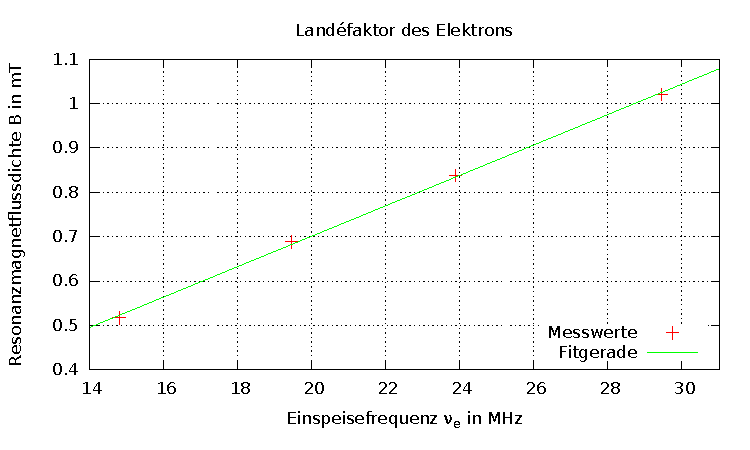
\includegraphics[width=0.8\textwidth]{../pics/landefaktor.pdf}
\caption{Gyromagnetisches Verhältnis oder Landéfaktor des Elektrons}
\label{pic_gyro}
\end{figure}
\noindent und zu einem Steigungsparameter 
\begin{equation}
m_\text{gyro} = 0,0343 \pm 0,0006 \text{ Ts}
\end{equation}
führt und damit schließlich den Landéfaktor berechnen lässt.
\begin{equation}
 g = \frac{h}{\mu_B\cdot m_\text{gyro}} = 2,082 \pm 0,037
\end{equation}


\section{Diskussion}
\subsection{Erdmagnetfeld}
Der berechnete Wert für das Erdmagnetfeld steht in folgendem Verhältnis zum Literaturwert \cite{ErdB}
\begin{equation}
 \frac{B_\text{Mess}}{B_\text{Lit}} = 68,3 \%.
\end{equation}
Die etwas hohe Abweichung spricht für eine unpräzise Ausrichtung der Helmholtzspule, was auf die sehr empfindliche Bussole zurückführbar ist, die
auf diverse andere elektrische Geräte reagiert.

\subsection{Landéfaktor}
Das gyromagnetische Verhältnis wurde durch einen Fit ermittelt und hat eine Übereinstimmung zum Literaturwert \cite{Gyro} von
\begin{equation}
 \frac{g_\text{Mess}}{g_\text{Lit}} = 103,4 \%.
\end{equation}
Unabhängig von den Abweichungen vom Erdmagnetfeld ist eine sehr gute Bestimmung des Landéfaktors gelungen. 



\begin{thebibliography}{xxxxxxxxxxxxxxxxx}
 \bibitem[Chemie.de]{ErdB}Form und Stärke des Erdmagnetfelds\\ \href{http://www.chemie.de/lexikon/Erdmagnetfeld.html#Form_und_St.C3.A4rke_des_Erdmagnetfeldes}{chemie.de/lexikon/Erdmagnetfeld}
 \bibitem[Universal Lexikon]{Gyro}Landé-Faktor\\ \href{http://universal\_lexikon.deacademic.com/144745/}{universal\_lexikon.deacademic.com/144745/}
 \bibitem[Versuchsanleitung]{}{Versuch V28 Elektronen-Spin-Resonanz }
\end{thebibliography}

% ========================================
%	Literaturverzeichnis
% ========================================

%\bibliographystyle{plainnat}			% Bibliographie-Style auswählen
%\bibliography{BIBDATEI}			% Literaturverzeichnis

% ========================================
%	Das Dokument endent
% ========================================

\end{document}
